% ==============================================================================
% CHAPTER 7: BACKPROPAGATION
% ==============================================================================

\chapter{Backpropagation}
\label{ch:backpropagation}

\begin{keyconcept}
Backpropagation is the algorithm at the \textbf{heart of deep learning}. It enables neural networks to learn by efficiently computing gradients of the loss function with respect to all parameters. The heart of backpropagation is the \textbf{chain rule} of calculus.
\end{keyconcept}

% ------------------------------------------------------------------------------
\section{Motivation and Overview}
% ------------------------------------------------------------------------------

When training a neural network, we have:
\begin{itemize}
    \item A \textbf{loss function} $\mathcal{L}$ that measures how far our predictions are from the targets
    \item \textbf{Parameters} $\theta = \{W^{(1)}, b^{(1)}, W^{(2)}, b^{(2)}, \ldots, W^{(L)}, b^{(L)}\}$ that we can adjust
    \item The goal: adjust $\theta$ to minimize $\mathcal{L}$
\end{itemize}

To use gradient descent, we need $\frac{\partial \mathcal{L}}{\partial W^{(k)}}$ and $\frac{\partial \mathcal{L}}{\partial b^{(k)}}$ for all layers $k$. Backpropagation provides an efficient way to compute these gradients.

\subsection{Independent vs. Dependent Parameters}

\begin{infobox}{What Can We Actually Change?}
When inspecting a neural network, we can categorize quantities into:
\begin{itemize}
    \item \textbf{Fixed inputs}: The data $X$ is given; we cannot change it
    \item \textbf{Dependent parameters}: Hidden activations $h^{(k)}$, pre-activations $a^{(k)}$---these are \emph{effects} that happen because of other causes
    \item \textbf{Independent parameters}: Weights $W^{(k)}$ and biases $b^{(k)}$---these are the \emph{causes} that we have control over
\end{itemize}
The only quantities we can directly adjust are the \textbf{weights and biases}. Everything else is a consequence of these choices.
\end{infobox}

% ------------------------------------------------------------------------------
\section{Review of Calculus Fundamentals}
% ------------------------------------------------------------------------------

\subsection{The Derivative as Rate of Change}

For a univariate function $y = f(x)$, the derivative tells us how a small change in $x$ affects $y$:
\[
\frac{dy}{dx} = \lim_{\Delta x \to 0} \frac{f(x + \Delta x) - f(x)}{\Delta x}
\]

If we nudge $x$ by a small amount $\Delta x$, then:
\[
\Delta y \approx \frac{dy}{dx} \cdot \Delta x
\]

\subsection{Partial Derivatives and Multivariate Functions}

For a function $y = f(x_1, x_2, \ldots, x_m)$ with multiple inputs, we use \textbf{partial derivatives}:
\[
\frac{\partial y}{\partial x_i} = \text{rate of change of } y \text{ when only } x_i \text{ changes (others held constant)}
\]

\begin{boxed}
\textbf{Influence Diagram for Multivariate Functions} \\[1em]
\begin{center}
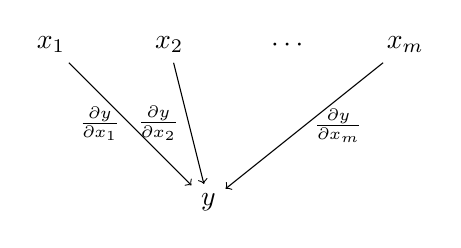
\begin{tikzpicture}[node distance=1.5cm, auto]
    \node (x1) {$x_1$};
    \node (x2) [right of=x1] {$x_2$};
    \node (dots) [right of=x2] {$\cdots$};
    \node (xm) [right of=dots] {$x_m$};
    \node (y) [below of=x2, xshift=0.5cm, yshift=-0.5cm] {$y$};
    
    \draw[->] (x1) -- node[left, font=\footnotesize] {$\frac{\partial y}{\partial x_1}$} (y);
    \draw[->] (x2) -- node[left, font=\footnotesize] {$\frac{\partial y}{\partial x_2}$} (y);
    \draw[->] (xm) -- node[right, font=\footnotesize] {$\frac{\partial y}{\partial x_m}$} (y);
\end{tikzpicture}
\end{center}
\end{boxed}

The \textbf{total change} in $y$ when all inputs change:
\[
\Delta y = \sum_{i=1}^{m} \frac{\partial y}{\partial x_i} \Delta x_i
\]

\subsection{The Chain Rule}

For composed (nested) functions $y = f(g(x))$, we have:
\[
\frac{dy}{dx} = \frac{dy}{dg} \cdot \frac{dg}{dx}
\]

\begin{derivation}{Chain Rule for Nested Functions}
Let $y = f(g(x))$. If we nudge $x$ by $\Delta x$:
\begin{enumerate}
    \item First, $g$ changes: $\Delta g = \frac{dg}{dx} \cdot \Delta x$
    \item Then, $y$ changes: $\Delta y = \frac{dy}{dg} \cdot \Delta g$
    \item Substituting: $\Delta y = \frac{dy}{dg} \cdot \frac{dg}{dx} \cdot \Delta x$
\end{enumerate}
Therefore: $\boxed{\frac{dy}{dx} = \frac{dy}{dg} \cdot \frac{dg}{dx}}$
\end{derivation}

\subsection{Chain Rule with Multiple Paths}

For $y = f(z_1, z_2, \ldots, z_m)$ where each $z_i = g_i(x)$:
\[
\frac{\partial y}{\partial x} = \sum_{i=1}^{m} \frac{\partial y}{\partial z_i} \cdot \frac{\partial z_i}{\partial x}
\]

\begin{important}
This is the \textbf{key insight for neural networks}: when one variable influences the output through multiple paths, we must \textbf{sum the contributions} from all paths.
\end{important}

% ------------------------------------------------------------------------------
\section{Computational Graphs}
% ------------------------------------------------------------------------------

A \textbf{computational graph} represents the computation as a directed acyclic graph (DAG) where:
\begin{itemize}
    \item \textbf{Nodes} represent values (inputs, intermediate results, outputs)
    \item \textbf{Edges} represent operations that produce one value from others
\end{itemize}

\begin{example}
Consider $\mathcal{L} = (a + b) \times c$. The computational graph is:

\begin{center}
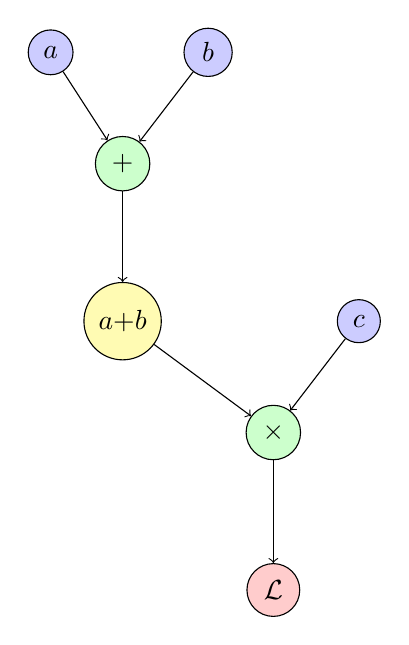
\begin{tikzpicture}[node distance=2cm, auto]
    \node[circle, draw, fill=blue!20] (a) {$a$};
    \node[circle, draw, fill=blue!20] (b) [right of=a] {$b$};
    \node[circle, draw, fill=green!20] (plus) [below right of=a, xshift=-0.5cm] {$+$};
    \node[circle, draw, fill=yellow!30] (ab) [below of=plus] {$a{+}b$};
    \node[circle, draw, fill=blue!20] (c) [right of=ab, xshift=1cm] {$c$};
    \node[circle, draw, fill=green!20] (mult) [below right of=ab, xshift=0.5cm] {$\times$};
    \node[circle, draw, fill=red!20] (L) [below of=mult] {$\mathcal{L}$};
    
    \draw[->] (a) -- (plus);
    \draw[->] (b) -- (plus);
    \draw[->] (plus) -- (ab);
    \draw[->] (ab) -- (mult);
    \draw[->] (c) -- (mult);
    \draw[->] (mult) -- (L);
\end{tikzpicture}
\end{center}

To find $\frac{\partial \mathcal{L}}{\partial a}$, we trace the path from $\mathcal{L}$ back to $a$:
\[
\frac{\partial \mathcal{L}}{\partial a} = \frac{\partial \mathcal{L}}{\partial (a+b)} \cdot \frac{\partial (a+b)}{\partial a} = c \cdot 1 = c
\]
\end{example}

% ------------------------------------------------------------------------------
\section{Forward Pass: Notation and Review}
% ------------------------------------------------------------------------------

\subsection{Notation Summary}

For a neural network with $L$ layers:
\begin{itemize}
    \item $n_k$ = number of neurons in layer $k$
    \item $W^{(k)} \in \mathbb{R}^{n_k \times n_{k-1}}$ = weight matrix connecting layer $k-1$ to layer $k$
    \item $b^{(k)} \in \mathbb{R}^{n_k}$ = bias vector for layer $k$
    \item $a^{(k)} \in \mathbb{R}^{n_k}$ = pre-activation (affine transformation) at layer $k$
    \item $h^{(k)} \in \mathbb{R}^{n_k}$ = post-activation (hidden output) at layer $k$
    \item $f$ = activation function (e.g., sigmoid, ReLU)
    \item $h^{(0)} = X$ (input)
    \item $h^{(L)} = \hat{Y}$ (prediction)
\end{itemize}

\subsection{Forward Pass Equations}

\textbf{Vector Form:}
\begin{align}
a^{(k)} &= W^{(k)} h^{(k-1)} + b^{(k)} \label{eq:forward_affine} \\
h^{(k)} &= f(a^{(k)}) \label{eq:forward_activation}
\end{align}

\textbf{Element-wise Form:}
\begin{align}
a_i^{(k)} &= \sum_{j=1}^{n_{k-1}} W_{ij}^{(k)} h_j^{(k-1)} + b_i^{(k)} \\
h_i^{(k)} &= f(a_i^{(k)})
\end{align}

where $W_{ij}^{(k)}$ is the weight connecting neuron $j$ in layer $k-1$ to neuron $i$ in layer $k$.

% ------------------------------------------------------------------------------
\section{The Error (Delta) Vector}
% ------------------------------------------------------------------------------

To simplify backpropagation calculations, we define the \textbf{error vector} (also called \textbf{delta} or \textbf{blame vector}):

\begin{definition}[Error Vector]
The error at layer $k$ is defined as:
\[
\boxed{\delta^{(k)} = \frac{\partial \mathcal{L}}{\partial a^{(k)}}}
\]

Element-wise:
\[
\delta_i^{(k)} = \frac{\partial \mathcal{L}}{\partial a_i^{(k)}}
\]
\end{definition}

\textbf{Interpretation}: $\delta_i^{(k)}$ tells us how much neuron $i$ in layer $k$ is ``to blame'' for the loss. It quantifies how much a small change in the pre-activation $a_i^{(k)}$ would affect the loss.

% ------------------------------------------------------------------------------
\section{Backpropagation Derivation}
% ------------------------------------------------------------------------------

\subsection{Step 1: Error at the Output Layer}

At the output layer $L$, we compute the error using the chain rule:

\begin{derivation}{Output Layer Error $\delta^{(L)}$}
We want $\delta^{(L)} = \frac{\partial \mathcal{L}}{\partial a^{(L)}}$.

By chain rule, since $\mathcal{L}$ depends on $a^{(L)}$ through $h^{(L)} = f(a^{(L)})$:
\[
\delta_i^{(L)} = \frac{\partial \mathcal{L}}{\partial a_i^{(L)}} = \frac{\partial \mathcal{L}}{\partial h_i^{(L)}} \cdot \frac{\partial h_i^{(L)}}{\partial a_i^{(L)}}
\]

Since $h_i^{(L)} = f(a_i^{(L)})$, we have $\frac{\partial h_i^{(L)}}{\partial a_i^{(L)}} = f'(a_i^{(L)})$.

\textbf{Element-wise form:}
\[
\boxed{\delta_i^{(L)} = \frac{\partial \mathcal{L}}{\partial h_i^{(L)}} \cdot f'(a_i^{(L)})}
\]

\textbf{Vector form:}
\[
\boxed{\delta^{(L)} = \frac{\partial \mathcal{L}}{\partial h^{(L)}} \odot f'(a^{(L)})}
\]
where $\odot$ denotes the Hadamard (element-wise) product.
\end{derivation}

\subsubsection{Common Loss Functions}

For \textbf{Mean Squared Error} loss $\mathcal{L} = \frac{1}{2}\|h^{(L)} - y\|^2$:
\[
\frac{\partial \mathcal{L}}{\partial h^{(L)}} = h^{(L)} - y
\]

For \textbf{Cross-Entropy with Softmax} output:
\[
\delta^{(L)} = h^{(L)} - y \quad \text{(a remarkably simple result!)}
\]

\subsection{Step 2: Backpropagating the Error}

For hidden layers $k = L-1, L-2, \ldots, 1$, we propagate the error backwards.

\begin{derivation}{Hidden Layer Error $\delta^{(k)}$}
Consider neuron $i$ in layer $k$. Its pre-activation $a_i^{(k)}$ affects the loss through \emph{all neurons in layer $k+1$}:

\begin{center}
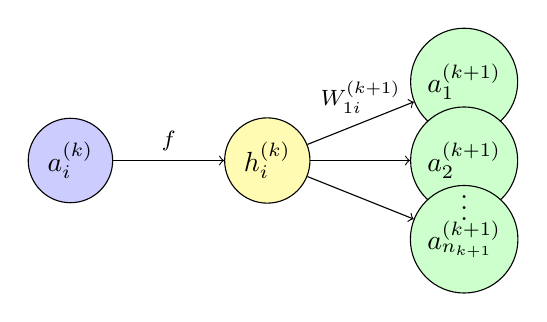
\begin{tikzpicture}[node distance=2.5cm, auto]
    \node[circle, draw, fill=blue!20] (ai) {$a_i^{(k)}$};
    \node[circle, draw, fill=yellow!30] (hi) [right of=ai] {$h_i^{(k)}$};
    \node[circle, draw, fill=green!20] (a1) [right of=hi, yshift=1cm] {$a_1^{(k+1)}$};
    \node[circle, draw, fill=green!20] (a2) [right of=hi] {$a_2^{(k+1)}$};
    \node[circle, draw, fill=green!20] (an) [right of=hi, yshift=-1cm] {$a_{n_{k+1}}^{(k+1)}$};
    \node (dots) [right of=hi, yshift=-0.5cm] {$\vdots$};
    
    \draw[->] (ai) -- node[above, font=\footnotesize] {$f$} (hi);
    \draw[->] (hi) -- node[above, font=\footnotesize] {$W_{1i}^{(k+1)}$} (a1);
    \draw[->] (hi) -- (a2);
    \draw[->] (hi) -- (an);
\end{tikzpicture}
\end{center}

By the chain rule with multiple paths:
\begin{align}
\delta_i^{(k)} &= \frac{\partial \mathcal{L}}{\partial a_i^{(k)}} \\
&= \frac{\partial \mathcal{L}}{\partial h_i^{(k)}} \cdot \frac{\partial h_i^{(k)}}{\partial a_i^{(k)}} \\
&= \left( \sum_{\ell=1}^{n_{k+1}} \frac{\partial \mathcal{L}}{\partial a_\ell^{(k+1)}} \cdot \frac{\partial a_\ell^{(k+1)}}{\partial h_i^{(k)}} \right) \cdot f'(a_i^{(k)})
\end{align}

Since $a_\ell^{(k+1)} = \sum_j W_{\ell j}^{(k+1)} h_j^{(k)} + b_\ell^{(k+1)}$, we have:
\[
\frac{\partial a_\ell^{(k+1)}}{\partial h_i^{(k)}} = W_{\ell i}^{(k+1)}
\]

Therefore:
\[
\boxed{\delta_i^{(k)} = f'(a_i^{(k)}) \cdot \sum_{\ell=1}^{n_{k+1}} W_{\ell i}^{(k+1)} \delta_\ell^{(k+1)}}
\]

\textbf{Vector form:}
\[
\boxed{\delta^{(k)} = \left( W^{(k+1)^\top} \delta^{(k+1)} \right) \odot f'(a^{(k)})}
\]
\end{derivation}

\subsection{Step 3: Gradients with Respect to Parameters}

Now we compute the gradients with respect to weights and biases.

\begin{derivation}{Gradient with Respect to Weights}
Consider weight $W_{ij}^{(k)}$ connecting $h_j^{(k-1)}$ to $a_i^{(k)}$:

Since $a_i^{(k)} = \sum_j W_{ij}^{(k)} h_j^{(k-1)} + b_i^{(k)}$:
\[
\frac{\partial a_i^{(k)}}{\partial W_{ij}^{(k)}} = h_j^{(k-1)}
\]

By chain rule:
\[
\frac{\partial \mathcal{L}}{\partial W_{ij}^{(k)}} = \frac{\partial \mathcal{L}}{\partial a_i^{(k)}} \cdot \frac{\partial a_i^{(k)}}{\partial W_{ij}^{(k)}} = \delta_i^{(k)} \cdot h_j^{(k-1)}
\]

\textbf{Element-wise form:}
\[
\boxed{\frac{\partial \mathcal{L}}{\partial W_{ij}^{(k)}} = \delta_i^{(k)} \cdot h_j^{(k-1)}}
\]

\textbf{Matrix form:}
\[
\boxed{\frac{\partial \mathcal{L}}{\partial W^{(k)}} = \delta^{(k)} \cdot h^{(k-1)^\top}}
\]
\end{derivation}

\begin{derivation}{Gradient with Respect to Biases}
Since $a_i^{(k)} = \sum_j W_{ij}^{(k)} h_j^{(k-1)} + b_i^{(k)}$:
\[
\frac{\partial a_i^{(k)}}{\partial b_i^{(k)}} = 1
\]

Therefore:
\[
\boxed{\frac{\partial \mathcal{L}}{\partial b_i^{(k)}} = \delta_i^{(k)}}
\]

\textbf{Vector form:}
\[
\boxed{\frac{\partial \mathcal{L}}{\partial b^{(k)}} = \delta^{(k)}}
\]
\end{derivation}

% ------------------------------------------------------------------------------
\section{Summary: The Backpropagation Algorithm}
% ------------------------------------------------------------------------------

\begin{algorithm}[Backpropagation]
\textbf{Input:} Training example $(X, y)$, network parameters $\{W^{(k)}, b^{(k)}\}_{k=1}^L$

\textbf{Forward Pass:}
\begin{enumerate}
    \item Set $h^{(0)} = X$
    \item For $k = 1, 2, \ldots, L$:
    \begin{itemize}
        \item Compute $a^{(k)} = W^{(k)} h^{(k-1)} + b^{(k)}$ \hfill (cache $a^{(k)}$)
        \item Compute $h^{(k)} = f(a^{(k)})$ \hfill (cache $h^{(k)}$)
    \end{itemize}
    \item Compute loss $\mathcal{L}(h^{(L)}, y)$
\end{enumerate}

\textbf{Backward Pass:}
\begin{enumerate}
    \item Compute output error: $\delta^{(L)} = \frac{\partial \mathcal{L}}{\partial h^{(L)}} \odot f'(a^{(L)})$
    \item For $k = L-1, L-2, \ldots, 1$:
    \begin{itemize}
        \item Compute $\delta^{(k)} = \left( W^{(k+1)^\top} \delta^{(k+1)} \right) \odot f'(a^{(k)})$
    \end{itemize}
    \item Compute gradients for all layers: \\
    $\frac{\partial \mathcal{L}}{\partial W^{(k)}} = \delta^{(k)} \cdot h^{(k-1)^\top}$ \quad and \quad $\frac{\partial \mathcal{L}}{\partial b^{(k)}} = \delta^{(k)}$
\end{enumerate}
\end{algorithm}

% ------------------------------------------------------------------------------
\section{Worked Example: Backpropagation by Hand}
% ------------------------------------------------------------------------------

Let us perform one complete forward and backward pass on a small network.

\subsection{Network Setup}

\begin{itemize}
    \item \textbf{Architecture}: 2 inputs $\to$ 2 hidden $\to$ 2 hidden $\to$ 2 outputs
    \item \textbf{Activation}: Sigmoid throughout
    \item \textbf{Loss}: Mean Squared Error
\end{itemize}

\textbf{Weight Matrices:}
\[
W^{(1)} = \begin{pmatrix} 0.1 & 0.2 \\ 0.3 & 0.4 \end{pmatrix}, \quad
W^{(2)} = \begin{pmatrix} 0.5 & 0.6 \\ 0.7 & 0.8 \end{pmatrix}, \quad
W^{(3)} = \begin{pmatrix} 0.9 & 1.0 \\ 1.1 & 1.2 \end{pmatrix}
\]

\textbf{Bias Vectors:}
\[
b^{(1)} = b^{(2)} = b^{(3)} = \begin{pmatrix} 0.1 \\ 0.1 \end{pmatrix}
\]

\textbf{Training Example:}
\[
X = h^{(0)} = \begin{pmatrix} 1 \\ 0 \end{pmatrix}, \qquad y = \begin{pmatrix} 0 \\ 1 \end{pmatrix}
\]

\subsection{Forward Pass}

\textbf{Layer 1:}
\begin{align}
a^{(1)} &= W^{(1)} h^{(0)} + b^{(1)} = \begin{pmatrix} 0.1 & 0.2 \\ 0.3 & 0.4 \end{pmatrix} \begin{pmatrix} 1 \\ 0 \end{pmatrix} + \begin{pmatrix} 0.1 \\ 0.1 \end{pmatrix} = \begin{pmatrix} 0.2 \\ 0.4 \end{pmatrix} \\
h^{(1)} &= \sigma(a^{(1)}) = \begin{pmatrix} \sigma(0.2) \\ \sigma(0.4) \end{pmatrix} = \begin{pmatrix} 0.550 \\ 0.599 \end{pmatrix}
\end{align}

\textbf{Layer 2:}
\begin{align}
a^{(2)} &= W^{(2)} h^{(1)} + b^{(2)} = \begin{pmatrix} 0.5(0.550) + 0.6(0.599) + 0.1 \\ 0.7(0.550) + 0.8(0.599) + 0.1 \end{pmatrix} = \begin{pmatrix} 0.734 \\ 0.964 \end{pmatrix} \\
h^{(2)} &= \sigma(a^{(2)}) = \begin{pmatrix} 0.676 \\ 0.724 \end{pmatrix}
\end{align}

\textbf{Layer 3 (Output):}
\begin{align}
a^{(3)} &= W^{(3)} h^{(2)} + b^{(3)} = \begin{pmatrix} 0.9(0.676) + 1.0(0.724) + 0.1 \\ 1.1(0.676) + 1.2(0.724) + 0.1 \end{pmatrix} = \begin{pmatrix} 1.432 \\ 1.712 \end{pmatrix} \\
h^{(3)} &= \sigma(a^{(3)}) = \begin{pmatrix} 0.807 \\ 0.847 \end{pmatrix}
\end{align}

\textbf{Loss:}
\[
\mathcal{L} = \frac{1}{2}\|h^{(3)} - y\|^2 = \frac{1}{2}\left[(0.807-0)^2 + (0.847-1)^2\right] = \frac{1}{2}(0.651 + 0.023) = 0.337
\]

\subsection{Backward Pass}

\textbf{Output Layer Error $\delta^{(3)}$:}

For MSE loss and sigmoid activation:
\begin{align}
\delta^{(3)} &= (h^{(3)} - y) \odot \sigma'(a^{(3)}) \\
&= \begin{pmatrix} 0.807 - 0 \\ 0.847 - 1 \end{pmatrix} \odot \begin{pmatrix} \sigma(1.432)(1-\sigma(1.432)) \\ \sigma(1.712)(1-\sigma(1.712)) \end{pmatrix} \\
&= \begin{pmatrix} 0.807 \\ -0.153 \end{pmatrix} \odot \begin{pmatrix} 0.156 \\ 0.130 \end{pmatrix} = \begin{pmatrix} 0.126 \\ -0.020 \end{pmatrix}
\end{align}

\textbf{Hidden Layer Error $\delta^{(2)}$:}
\begin{align}
\delta^{(2)} &= \left( W^{(3)^\top} \delta^{(3)} \right) \odot \sigma'(a^{(2)}) \\
&= \begin{pmatrix} 0.9 & 1.1 \\ 1.0 & 1.2 \end{pmatrix} \begin{pmatrix} 0.126 \\ -0.020 \end{pmatrix} \odot \begin{pmatrix} 0.219 \\ 0.200 \end{pmatrix} \\
&= \begin{pmatrix} 0.091 \\ 0.102 \end{pmatrix} \odot \begin{pmatrix} 0.219 \\ 0.200 \end{pmatrix} = \begin{pmatrix} 0.020 \\ 0.020 \end{pmatrix}
\end{align}

\textbf{Hidden Layer Error $\delta^{(1)}$:}
\begin{align}
\delta^{(1)} &= \left( W^{(2)^\top} \delta^{(2)} \right) \odot \sigma'(a^{(1)}) \\
&\approx \begin{pmatrix} 0.006 \\ 0.007 \end{pmatrix}
\end{align}

\textbf{Key Observation}: The errors \textbf{dilute as they propagate backwards}. This is why deep networks can suffer from the \emph{vanishing gradient problem}.

\subsection{Parameter Gradients}

\textbf{Gradients for $W^{(3)}$:}
\[
\frac{\partial \mathcal{L}}{\partial W^{(3)}} = \delta^{(3)} \cdot h^{(2)^\top} = \begin{pmatrix} 0.126 \\ -0.020 \end{pmatrix} \begin{pmatrix} 0.676 & 0.724 \end{pmatrix} = \begin{pmatrix} 0.085 & 0.091 \\ -0.014 & -0.015 \end{pmatrix}
\]

\textbf{Gradients for $b^{(3)}$:}
\[
\frac{\partial \mathcal{L}}{\partial b^{(3)}} = \delta^{(3)} = \begin{pmatrix} 0.126 \\ -0.020 \end{pmatrix}
\]

\subsection{Gradient Descent Update}

With learning rate $\eta = 0.1$:
\begin{align}
W^{(3)}_{\text{new}} &= W^{(3)} - \eta \cdot \frac{\partial \mathcal{L}}{\partial W^{(3)}} \\
&= \begin{pmatrix} 0.9 & 1.0 \\ 1.1 & 1.2 \end{pmatrix} - 0.1 \cdot \begin{pmatrix} 0.085 & 0.091 \\ -0.014 & -0.015 \end{pmatrix} \\
&= \begin{pmatrix} 0.891 & 0.991 \\ 1.101 & 1.202 \end{pmatrix}
\end{align}

% ------------------------------------------------------------------------------
\section{Mini-batch Gradient Descent}
% ------------------------------------------------------------------------------

In practice, we don't update after each example. Instead:

\begin{enumerate}
    \item \textbf{Shuffle} the dataset
    \item \textbf{Divide} into mini-batches of size $m$ (e.g., 32, 64, 128)
    \item For each mini-batch:
    \begin{itemize}
        \item Compute gradients for each example
        \item \textbf{Average} the gradients across the batch:
        \[
        \frac{\partial \mathcal{L}}{\partial W^{(k)}} = \frac{1}{m} \sum_{i=1}^{m} \frac{\partial \mathcal{L}_i}{\partial W^{(k)}}
        \]
        \item Update parameters using the averaged gradient
    \end{itemize}
\end{enumerate}

\begin{infobox}{Why Mini-batches?}
\begin{itemize}
    \item Computing gradients for all examples (batch gradient descent) is too slow
    \item Single-example updates (stochastic gradient descent) are too noisy
    \item Mini-batches provide a \textbf{balance}: reasonably accurate gradient estimates with computational efficiency
    \item The ``stochastic'' navigation of the loss landscape can help escape local minima
\end{itemize}
\end{infobox}

% ------------------------------------------------------------------------------
\section{Why is it Called ``Backpropagation''?}
% ------------------------------------------------------------------------------

The name comes from the fact that:
\begin{enumerate}
    \item Errors are computed starting from the \textbf{output layer}
    \item Errors are \textbf{propagated backwards} through the network
    \item To compute $\delta^{(k)}$, we need $\delta^{(k+1)}$, which comes ``after'' layer $k$ in the forward direction
\end{enumerate}

\begin{keyconcept}
Backpropagation is an efficient implementation of the chain rule. It computes all gradients in $O(n)$ time (where $n$ is the number of parameters) by:
\begin{enumerate}
    \item \textbf{Caching} intermediate values during the forward pass
    \item \textbf{Reusing} error computations during the backward pass
\end{enumerate}
Without this caching, naive gradient computation would be exponentially expensive.
\end{keyconcept}

% ------------------------------------------------------------------------------
\section{Sigmoid Derivative}
% ------------------------------------------------------------------------------

For the sigmoid function $\sigma(x) = \frac{1}{1 + e^{-x}}$, the derivative has a beautiful form:

\begin{derivation}{Sigmoid Derivative}
\begin{align}
\sigma'(x) &= \frac{d}{dx}\left(\frac{1}{1 + e^{-x}}\right) \\
&= \frac{e^{-x}}{(1 + e^{-x})^2} \\
&= \frac{1}{1 + e^{-x}} \cdot \frac{e^{-x}}{1 + e^{-x}} \\
&= \sigma(x) \cdot \frac{(1 + e^{-x}) - 1}{1 + e^{-x}} \\
&= \sigma(x) \cdot (1 - \sigma(x))
\end{align}

\[
\boxed{\sigma'(x) = \sigma(x)(1 - \sigma(x))}
\]
\end{derivation}

This is computationally convenient because if we've already computed $\sigma(x)$ during the forward pass, we can compute the derivative without any additional exponentiations!

% ------------------------------------------------------------------------------
\section{Key Takeaways}
% ------------------------------------------------------------------------------

\begin{summary}
\textbf{Core Ideas:}
\begin{itemize}
    \item Backpropagation efficiently computes $\frac{\partial \mathcal{L}}{\partial W^{(k)}}$ and $\frac{\partial \mathcal{L}}{\partial b^{(k)}}$ for all layers
    \item The heart of backpropagation is the \textbf{chain rule} of calculus
    \item We define the \textbf{error vector} $\delta^{(k)} = \frac{\partial \mathcal{L}}{\partial a^{(k)}}$ to simplify calculations
\end{itemize}

\textbf{Key Equations:}
\begin{align}
\delta^{(L)} &= \frac{\partial \mathcal{L}}{\partial h^{(L)}} \odot f'(a^{(L)}) && \text{(output layer)} \\
\delta^{(k)} &= \left( W^{(k+1)^\top} \delta^{(k+1)} \right) \odot f'(a^{(k)}) && \text{(hidden layers)} \\
\frac{\partial \mathcal{L}}{\partial W^{(k)}} &= \delta^{(k)} \cdot h^{(k-1)^\top} && \text{(weight gradients)} \\
\frac{\partial \mathcal{L}}{\partial b^{(k)}} &= \delta^{(k)} && \text{(bias gradients)}
\end{align}
\end{summary}
